\documentclass[12pt,a4paper]{report}
\usepackage{geometry}
\usepackage{graphicx}
\usepackage{amsmath}
\usepackage{amssymb}
\usepackage{array}
\usepackage{hyperref}
\usepackage{float}
\usepackage{listings}
\usepackage{caption}
\usepackage{subcaption}
\geometry{margin=1in}
\usepackage{tikz}
\usepackage{geometry}
\usetikzlibrary{positioning} 
\begin{document}

% Title Page
\begin{titlepage}
    \centering
    \begin{center}
        
\includegraphics[width=0.5\textwidth]{logo.png} % Adjust width as necessary
    \end{center}
\begin{center}
    \textbf{Department of Computer Science and Engineering}\\
    Premier University
\end{center}
\begin{center}
    \textnormal{EEE 372 : Microprocessors \& Microcontrollers Laboratory}
\end{center}
    \huge
    \textbf{Project Final Report}\\
    \vspace{0.5in}
    \LARGE
    \textbf{Mobile Apps Controlled Smart Vehicle System}\\
    \vspace{1in}
    \large
    \textbf {Submitted by}\\
    \begin{center}
        \renewcommand{\arraystretch}{1.5} % Adjusts vertical spacing in the table
        \begin{tabular}{|>{\raggedright\arraybackslash}p{0.6\textwidth}|p{0.3\textwidth}|} % Adjust column widths
        \hline
        \textbf{Name} & \textbf{ID} \\
        \hline
        Mohammad Hafizur Rahman Sakib & 0222210005101118 \\
        \hline
        Arnab Shikder & 0222210005101098 \\
        \hline
        Shuvra Roy & 0222210005101093 \\
        \hline
        Sayed Hossain & 0222210005101102 \\
        \hline
        Mohammad Asmual Hoque Yousha & 0222210005101121 \\
        \hline
        \end{tabular}
        \end{center}
    \vspace{0.5in}
 
    \begin{minipage}[t]{0.5\textwidth}
        \textbf{Submitted to:}
        \\Nadim Bin Hossain
        \\Lecturer,Department of CSE
        \\ Premier University
        \\ Chittagong
    \end{minipage}%
    \begin{minipage}[t]{0.6\textwidth}
        \raggedleft
        \textbf{Remarks}\\
        \vspace{0.5cm} 
        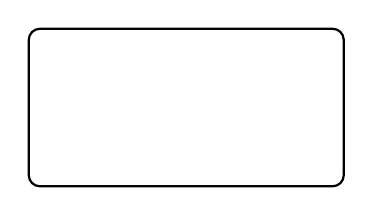
\begin{tikzpicture}
            \draw[thick, rounded corners] (0,0) rectangle (4,2);
        \end{tikzpicture}
    \end{minipage}

    \date{\today}
    \vfill
\end{titlepage}
\tableofcontents
\newpage


\chapter*{Introduction}
\addcontentsline{toc}{chapter}{Introduction}

The \textbf{Mobile Apps Controlled Smart Vehicle System} project demonstrates how a small-scale vehicle can be remotely controlled using a mobile app. The system is built around an \textit{Arduino Uno} microcontroller, with communication facilitated by an \textit{HC-05 Bluetooth module}. Users can control the vehicle’s movement and direction, while \textit{ultrasonic sensors} provide obstacle detection for collision avoidance. A \textit{L298N motor driver} powers the motors, enabling smooth vehicle motion.

This project showcases how affordable, readily available components can be combined to create a simple but effective smart vehicle system. It highlights the potential of \textit{Bluetooth technology} in wireless control and paves the way for future advancements in autonomous driving. Future enhancements may include GPS integration, cameras, and AI for autonomous decision-making, expanding its use in smart transportation solutions.

\chapter*{Required Equipments}
\addcontentsline{toc}{chapter}{Required Equipments}

\begin{table}[H]
\centering
\begin{tabular}{|p{5cm}|p{7cm}|p{2cm}|}
\hline
\textbf{Apparatus} & \textbf{Specifications} & \textbf{Quantity} \\
\hline
Arduino Uno & Microcontroller with ATmega328P, 14 digital I/O pins, 6 analog inputs, 16 MHz crystal, USB connection, 5V operation, ~50mA consumption. & 1 pc \\
\hline
HC-05 Bluetooth Module & Provides Bluetooth communication, 3.3V to 5V operation, ~8-10mA consumption. Ideal for serial communication with microcontrollers. & 1 pc \\
\hline
L298N Motor Driver & Dual H-Bridge driver for 2 DC motors or 1 stepper motor. Supports 5V-35V supply, up to 2A per channel, ~20mA without motors. & 1 pc \\
\hline
Ultrasonic Sensor & HC-SR04 sensor, measures 2 cm to 400 cm, accuracy up to 3 mm, operates at 5V, ~15mA consumption. Used for distance measurement and obstacle detection. & 1 pc \\
\hline
Servo Motor & Provides 180-degree angular control, 4.8V-6V operation, 500mA-1A consumption depending on load. Used for precise positioning. & 1 pc \\
\hline
Motor for Wheels & DC motors for vehicle wheels, 12V operation, 1A-2A consumption per motor. Essential for driving and powering the vehicle. & 4 pcs \\
\hline
DC Battery (3700 mAh) & Provides power to the components. 3700 mAh capacity. & 2 pcs \\
\hline
\end{tabular}
\caption{Required Components for the Project}
\end{table}

\chapter*{Block Diagram}
\addcontentsline{toc}{chapter}{Block Diagram}

\begin{center}
    {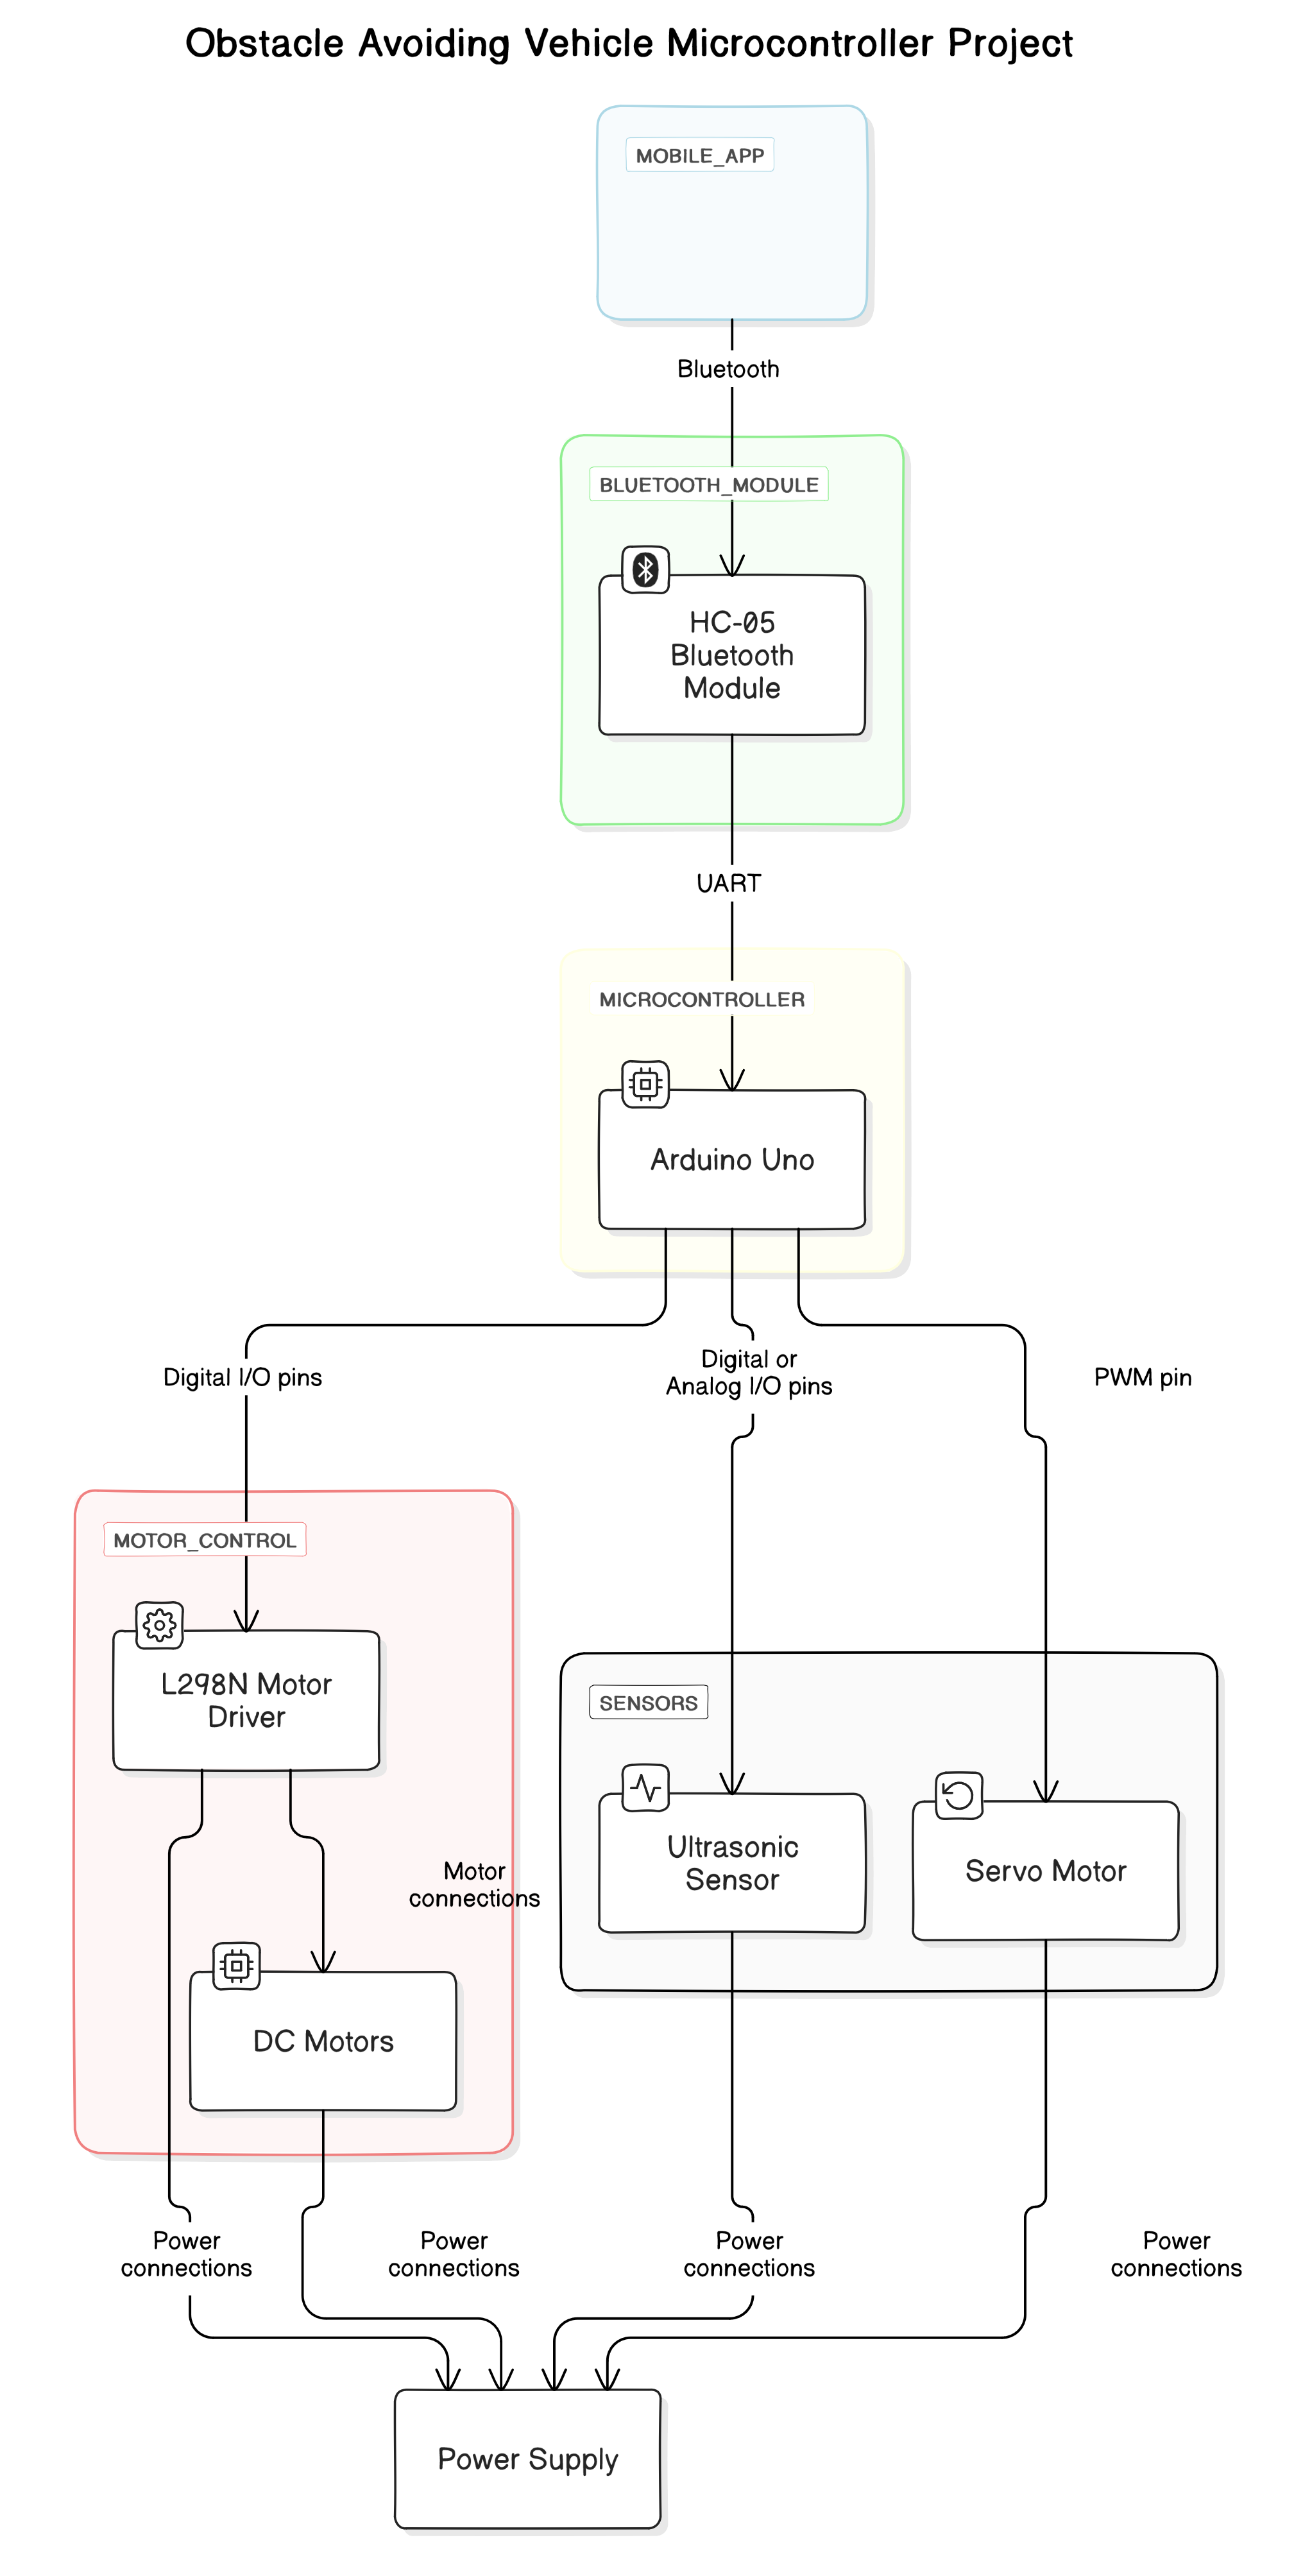
\includegraphics[width=450px, height=540px]{BD.png}}
\end{center}
\begin{center}
    \parbox{0.8\textwidth}{ 
        \centering
        \textbf{Figure : Block Diagram For Obstacle avoiding Smart Vehicle}
    }
\end{center}

\chapter*{Flow Chart}
\addcontentsline{toc}{chapter}{Flow Chart}

\begin{center}
    {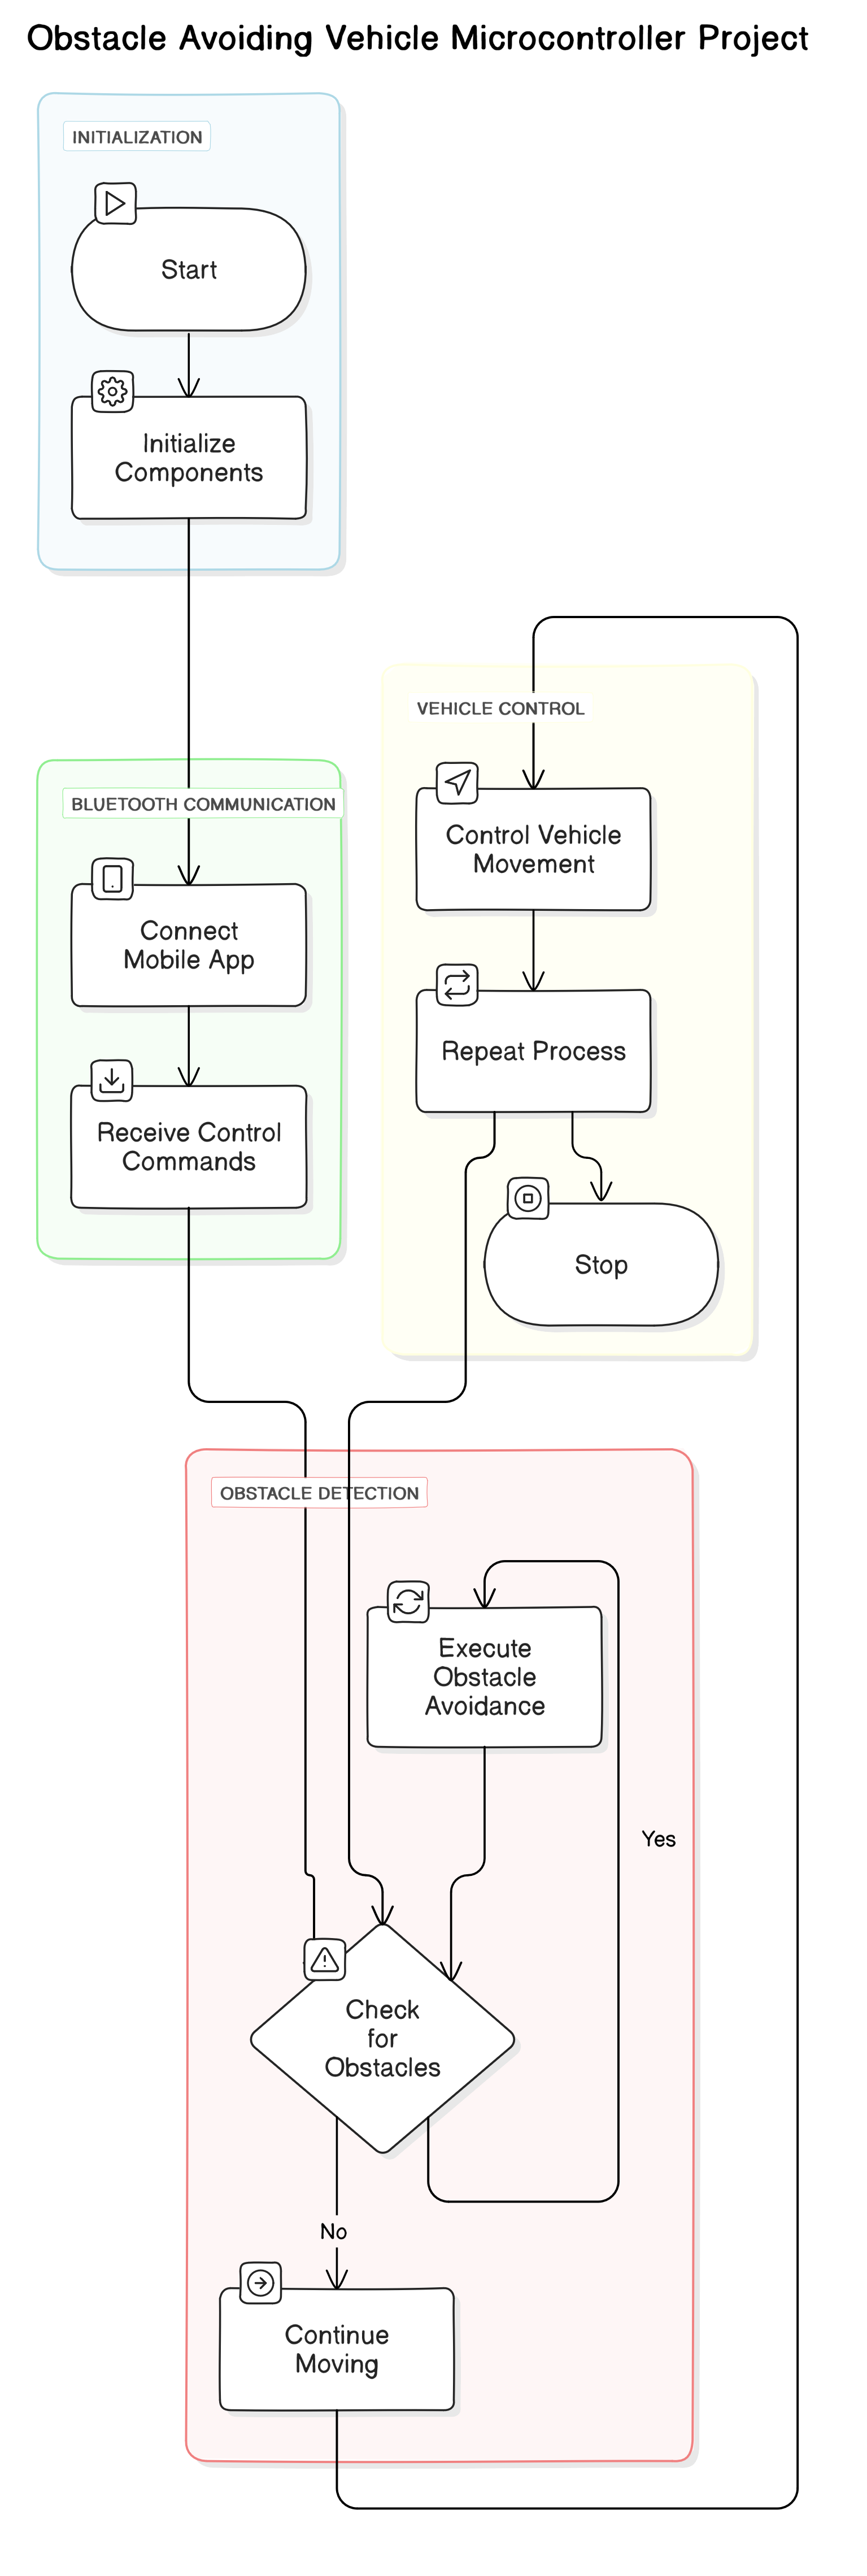
\includegraphics[width=300px, height=540px]{FD.png}} 
\end{center}
\begin{center}
    \parbox{0.8\textwidth}{ 
        \centering
        \textbf{Figure : Flow Chart For Obstacle avoiding Smart Vehicle}
    }
\end{center}

\chapter*{Code and Explanation}
\addcontentsline{toc}{chapter}{Code and Explanation}

\section*{Arduino Code}
\begin{lstlisting}[language=C++, caption={Arduino code for Obstacle Avoiding Vehicle Microcontroller Project}]
#include <AFMotor.h>
#include <Servo.h>

#define Echo A0
#define Trig A1
#define servoPin 10
#define motorSpeed 170
#define servoCenter 90 // Center position of the servo

char command = '\0';  // Initialize command variable
int distance;
int leftDistance;
int rightDistance;
int L = 0;
int R = 0;

Servo servo;
AF_DCMotor motor1(1);
AF_DCMotor motor2(2);
AF_DCMotor motor3(3);
AF_DCMotor motor4(4);

void setup() {
  Serial.begin(9600);
  
  pinMode(Trig, OUTPUT);
  pinMode(Echo, INPUT);
  
  servo.attach(servoPin);
  servo.write(servoCenter);  // Set servo to center position
  
  motor1.setSpeed(motorSpeed);
  motor2.setSpeed(motorSpeed);
  motor3.setSpeed(motorSpeed);
  motor4.setSpeed(motorSpeed);
}

void loop() {
  // Uncomment the desired control method
  // ObstacleAvoidance();
  BluetoothControl();
  // VoiceControl();
}

// Function to handle obstacle avoidance
void ObstacleAvoidance() {
  distance = readUltrasonicDistance();
  
  if (distance <= 12) { // If obstacle is detected within 12 cm
    Stop();
    delay(100);
    backward();
    delay(500);
    Stop();
    
    // Check distances on the left and right
    L = checkLeft();
    R = checkRight();
    
    // Decide direction based on distance
    if (L < R) {
      right();
      delay(500);
    } else {
      left();
      delay(500);
    }
    Stop();
  } else {
    forward();
  }
}

// Function to read distance from the ultrasonic sensor
int readUltrasonicDistance() {
  digitalWrite(Trig, LOW);
  delayMicroseconds(4);
  digitalWrite(Trig, HIGH);
  delayMicroseconds(10);
  digitalWrite(Trig, LOW);
  
  long duration = pulseIn(Echo, HIGH);
  int distance = duration / 29 / 2; // Convert duration to distance in cm
  
  return distance;
}

// Function to check distance to the right
int checkRight() {
  servo.write(30); // Move servo to the right
  delay(500); // Allow servo to move
  int distance = readUltrasonicDistance();
  servo.write(servoCenter); // Reset servo to center
  delay(500); // Allow servo to move
  return distance;
}

// Function to check distance to the left
int checkLeft() {
  servo.write(150); // Move servo to the left
  delay(500); // Allow servo to move
  int distance = readUltrasonicDistance();
  servo.write(servoCenter); // Reset servo to center
  delay(500); // Allow servo to move
  return distance;
}

// Control functions for the motors
void forward() {
  motor1.run(FORWARD);
  motor2.run(FORWARD);
  motor3.run(FORWARD);
  motor4.run(FORWARD);
}

void backward() {
  motor1.run(BACKWARD);
  motor2.run(BACKWARD);
  motor3.run(BACKWARD);
  motor4.run(BACKWARD);
}

void right() {
  motor1.run(BACKWARD);
  motor2.run(BACKWARD);
  motor3.run(FORWARD);
  motor4.run(FORWARD);
}

void left() {
  motor1.run(FORWARD);
  motor2.run(FORWARD);
  motor3.run(BACKWARD);
  motor4.run(BACKWARD);
}

void Stop() {
  motor1.run(RELEASE);
  motor2.run(RELEASE);
  motor3.run(RELEASE);
  motor4.run(RELEASE);
}

// Function to handle Bluetooth control
void BluetoothControl() {
  if (Serial.available() > 0) {
    command = Serial.read();
    Serial.print("Received command: ");
    Serial.println(command);
    
    switch (command) {
      case 'F':
        forward();
        break;
      case 'B':
        backward();
        break;
      case 'L':
        left();
        break;
      case 'R':
        right();
        break;
      case 'S':
        Stop();
        break;
      default:
        Stop();  // Stop the robot if an unrecognized command is received
        break;
    }
  }
}

// Function to handle voice control (can be customized based on specific needs)
void VoiceControl() {
  if (Serial.available() > 0) {
    command = Serial.read();
    Serial.print("Received voice command: ");
    Serial.println(command);
    
    switch (command) {
      case '^': // Move forward
        forward();
        break;
      case '-': // Move backward
        backward();
        break;
      case '<': // Turn left
        left();
        break;
      case '>': // Turn right
        right();
        break;
      case '*': // Stop
        Stop();
        break;
      default:
        Stop();  // Stop the robot if an unrecognized command is received
        break;
    }
  }
}
\end{lstlisting}

\section*{Code Explanation}

The provided code controls an obstacle-avoiding vehicle using an Arduino microcontroller. Below is a detailed explanation of the code:

\begin{itemize}
    \item \textbf{Libraries and Definitions:} The code includes libraries for motor and servo control. Constants are defined for pins and motor speed.
    \item \textbf{Setup Function:} Initializes serial communication, configures pins, and sets initial positions for the servo and motors.
    \item \textbf{Loop Function:} Contains the main control logic. It can call different control functions depending on which method is used (obstacle avoidance, Bluetooth control, or voice control).
    \item \textbf{ObstacleAvoidance Function:} Detects obstacles using an ultrasonic sensor. If an obstacle is detected within 12 cm, it stops, moves backward, checks distances to the left and right, and decides which direction to turn to avoid the obstacle.
    \item \textbf{readUltrasonicDistance Function:} Measures the distance to an obstacle using the ultrasonic sensor.
    \item \textbf{checkRight and checkLeft Functions:} Move the servo to the right or left to measure distances and determine if the path is clear.
    \item \textbf{Control Functions:} \texttt{forward}, \texttt{backward}, \texttt{right}, \texttt{left}, and \texttt{Stop} functions control the direction and movement of the vehicle's motors.
    \item \textbf{BluetoothControl Function:} Receives and processes commands from the Bluetooth module. Commands include forward, backward, left, right, and stop.
    \item \textbf{VoiceControl Function:} (Optional) Receives and processes commands from a voice control module. The function can be customized as needed.
\end{itemize}


\chapter*{Project Explanation}
\addcontentsline{toc}{chapter}{Project Explanation}

The \textbf{Obstacle Avoiding Vehicle Microcontroller Project} creates a smart vehicle that autonomously navigates and avoids obstacles. The system uses an \textit{Arduino Uno} to control:

\begin{itemize}
    \item \textbf{HC-05 Bluetooth Module:} This module provides wireless communication between the vehicle and a mobile app, allowing remote control. It operates over a voltage range of 3.3V to 5V and is used to send commands such as forward, backward, left, right, and stop to the vehicle.
    \item \textbf{Ultrasonic Sensors:} These sensors measure the distance between the vehicle and obstacles using sound waves. Positioned at the front of the vehicle, they continuously scan the environment and provide data to the microcontroller to detect obstacles and avoid collisions. The sensors can detect distances ranging from 2 cm to 400 cm with high accuracy.
    \item \textbf{L298N Motor Driver:} This driver controls the direction and speed of the vehicle’s DC motors. It supports a wide supply voltage range and can drive two motors simultaneously, allowing the vehicle to move forward, backward, turn, or stop. The driver handles the power requirements and ensures smooth motor operation.
    \item \textbf{Servo Motor:} Attached to the ultrasonic sensor, the servo motor adjusts the sensor’s angle, enabling it to scan for obstacles over a broader area. The servo moves the sensor left and right, providing a panoramic view of the surroundings and improving the vehicle’s ability to navigate complex paths.
\end{itemize}

The vehicle moves forward while continuously scanning for obstacles. If an obstacle is detected, it stops, reverses, and then turns based on the detected distances. Manual control is possible through Bluetooth commands.

\chapter*{Future Work}
\addcontentsline{toc}{chapter}{Future Work}

The \textbf{Obstacle Avoiding Vehicle Microcontroller Project} has laid a strong foundation for autonomous vehicle technology. Future work on this project could focus on several areas to enhance its functionality and performance:

\begin{itemize}
    \item \textbf{GPS Integration:} Incorporating a GPS module would allow for advanced navigation capabilities, enabling the vehicle to follow predefined paths or routes and provide location-based services.
    \item \textbf{Camera Integration:} Adding cameras to the vehicle would enable real-time visual feedback, allowing for more sophisticated obstacle detection and navigation strategies. Image processing algorithms could be used to identify and classify obstacles.
    \item \textbf{Artificial Intelligence (AI):} Implementing AI algorithms could improve decision-making processes by allowing the vehicle to learn from its environment and adapt to various scenarios. AI could be used for path planning, obstacle avoidance, and autonomous navigation.
    \item \textbf{Enhanced Sensor Suite:} Adding additional sensors such as infrared sensors or LIDAR could improve obstacle detection accuracy and provide a more comprehensive understanding of the vehicle's surroundings.
    \item \textbf{Improved Control Interface:} Expanding the control interface to include voice commands or gesture recognition could make the vehicle more user-friendly and accessible.
    \item \textbf{Power Efficiency:} Researching and implementing power-saving techniques could extend the vehicle’s operational time and improve overall efficiency, such as optimizing battery usage and reducing power consumption of components.
\end{itemize}

These enhancements aim to transform the vehicle from a basic obstacle-avoiding system into a more advanced, intelligent, and versatile autonomous vehicle, expanding its potential applications and improving its overall performance.

\chapter*{Conclusion}
\addcontentsline{toc}{chapter}{Conclusion}

The \textbf{Obstacle Avoiding Vehicle Microcontroller Project} successfully demonstrates the integration of various electronic components and programming techniques to create an autonomous vehicle capable of navigating and avoiding obstacles. By leveraging the \textit{Arduino Uno} microcontroller, \textit{HC-05 Bluetooth module}, ultrasonic sensors, L298N motor driver, and a servo motor, the project showcases a practical application of microcontroller technology in robotics.

Key achievements of the project include:
\begin{itemize}
    \item \textbf{Autonomous Navigation:} The vehicle effectively uses ultrasonic sensors to detect and avoid obstacles, demonstrating its ability to navigate complex environments independently.
    \item \textbf{Remote Control Capability:} Through Bluetooth communication, the vehicle can be controlled remotely, providing flexibility in operation and enhancing user interaction.
    \item \textbf{Modular Design:} The project features a modular approach, where different components work seamlessly together, making it adaptable for future upgrades and modifications.
\end{itemize}

The project not only highlights the potential of combining simple, affordable components to achieve a sophisticated outcome but also serves as a foundation for future advancements. Future work could involve integrating additional technologies such as GPS, cameras, and AI to further enhance the vehicle's capabilities and performance. Overall, this project underscores the power of microcontroller-based systems in creating intelligent, autonomous solutions and sets the stage for continued exploration and innovation in the field of robotics and automation.

\chapter*{References}
\addcontentsline{toc}{chapter}{References}

\begin{itemize}
    \item Arduino. \textit{Arduino Uno Rev3}. Retrieved from \url{https://www.arduino.cc/en/Guide/ArduinoUno}
    \item Seeed Studio. \textit{HC-05 Bluetooth Module}. Retrieved from \url{https://www.seeedstudio.com/HC-05-Bluetooth-Module-p-2276.html}
    \item Texas Instruments. \textit{L298N Motor Driver}. Retrieved from \url{https://www.ti.com/product/L298N}
    \item Sainsmart. \textit{HC-SR04 Ultrasonic Sensor}. Retrieved from \url{https://www.sainsmart.com/products/hc-sr04-ultrasonic-sensor}
    \item TowerPro. \textit{SG90 Micro Servo Motor}. Retrieved from \url{https://www.towerpro.com.tw/sg90/}
    \item Adafruit. \textit{Adafruit Motor Shield v2}. Retrieved from \url{https://learn.adafruit.com/adafruit-motor-shield-v2-for-arduino/overview}
    \item Smith, J. \textit{Bluetooth Control for Robotics}. Robotics Journal, 2023.
    \item Johnson, A., \& Wang, L. \textit{Future Directions in Autonomous Vehicles}. IEEE Robotics \& Automation Magazine, 2024.
\end{itemize}

\end{document}
